\documentclass[12pt]{report}
\usepackage[utf8]{inputenc}
\usepackage[russian]{babel}
\usepackage[14pt]{extsizes}
\usepackage{listings}
\usepackage{graphicx}
\usepackage{amsmath,amsfonts,amssymb,amsthm,mathtools} 
\usepackage{pgfplots}
\usepackage{filecontents}
\usepackage{float}
\usepackage{indentfirst}
\usepackage{eucal}
\usepackage{enumitem}
%s\documentclass[openany]{book}
\frenchspacing

\usepackage{titlesec}
\titleformat{\section}
{\normalsize\bfseries}
{\thesection}
{1em}{}
\titlespacing*{\chapter}{0pt}{-30pt}{8pt}
\titlespacing*{\section}{\parindent}{*4}{*4}
\titlespacing*{\subsection}{\parindent}{*4}{*4}

\usepackage{indentfirst} % Красная строка

\usetikzlibrary{datavisualization}
\usetikzlibrary{datavisualization.formats.functions}

\usepackage{amsmath}

\usepackage{amssymb}

% Для листинга кода:
\lstset{ %
	language=lisp,                 % выбор языка для подсветки (здесь это С)
	texcl=true,
	extendedchars=\true,
	basicstyle=\small\sffamily, % размер и начертание шрифта для подсветки кода
	numbers=left,               % где поставить нумерацию строк (слева\справа)
	numberstyle=\tiny,           % размер шрифта для номеров строк
	stepnumber=1,                   % размер шага между двумя номерами строк
	numbersep=5pt,                % как далеко отстоят номера строк от подсвечиваемого кода
	showspaces=false,            % показывать или нет пробелы специальными отступами
	showstringspaces=false,      % показывать или нет пробелы в строках
	showtabs=false,             % показывать или нет табуляцию в строках
	frame=single,              % рисовать рамку вокруг кода
	tabsize=2,                 % размер табуляции по умолчанию равен 2 пробелам
	captionpos=t,              % позиция заголовка вверху [t] или внизу [b] 
	breaklines=true,           % автоматически переносить строки (да\нет)
	breakatwhitespace=false, % переносить строки только если есть пробел
	escapeinside={\#*}{*)},  % если нужно добавить комментарии в коде
	%inputencoding=utf8x,
	%extendedchars=\true
}



\usepackage[left=2cm,right=2cm, top=2cm,bottom=2cm,bindingoffset=0cm]{geometry}
% Для измененных титулов глав:
\usepackage{titlesec, blindtext, color} % подключаем нужные пакеты
\definecolor{gray75}{gray}{0.75} % определяем цвет
\newcommand{\hsp}{\hspace{20pt}} % длина линии в 20pt
% titleformat определяет стиль
\titleformat{\chapter}[hang]{\Huge\bfseries}{\thechapter\hsp\textcolor{gray75}{|}\hsp}{0pt}{\Huge\bfseries}


% plot
\usepackage{pgfplots}
\usepackage{filecontents}
\usetikzlibrary{datavisualization}
\usetikzlibrary{datavisualization.formats.functions}

\begin{document}
	%\def\chaptername{} % убирает "Глава"
	\thispagestyle{empty}
	\begin{titlepage}
		\noindent \begin{minipage}{0.15\textwidth}
			
\includegraphics[width=\linewidth]{b_logo}
		\end{minipage}
		\noindent\begin{minipage}{0.9\textwidth}\centering
			\textbf{Министерство науки и высшего образования Российской Федерации}\\
			\textbf{Федеральное государственное бюджетное образовательное учреждение высшего образования}\\
			\textbf{~~~«Московский государственный технический университет имени Н.Э.~Баумана}\\
			\textbf{(национальный исследовательский университет)»}\\
			\textbf{(МГТУ им. Н.Э.~Баумана)}
		\end{minipage}
		
		\noindent\rule{18cm}{3pt}
		\newline\newline
		\noindent ФАКУЛЬТЕТ $\underline{\text{«Информатика и системы управления»}}$ \newline\newline
		\noindent КАФЕДРА $\underline{\text{«Программное обеспечение ЭВМ и информационные технологии»}}$\newline\newline\newline\newline\newline
		
		\begin{center}
			\noindent\begin{minipage}{1.1\textwidth}\centering
				\Large\textbf{  Отчет по лабораторной работе №8}\newline
				\textbf{по дисциплине <<Операционные системы>>}\newline
			\end{minipage}
		\end{center}
		
		\noindent\textbf{Тема} $\underline{\text{Системный вызов open()}}$\newline\newline
		\noindent\textbf{Студент} $\underline{\text{Золотухин А. В.~~~~~~~~~~~~~~~~~~~~~~~~~~~~~~~~~~~~~~~~~~}}$\newline\newline
		\noindent\textbf{Группа} $\underline{\text{ИУ7-64Б~~~~~~~~~~~~~~~~~~~~~~~~~~~~~~~~~~~~~~~~~~~~~~~~~~}}$\newline\newline
		\noindent\textbf{Оценка (баллы)} $\underline{\text{~~~~~~~~~~~~~~~~~~~~~~~~~~~~~~~~~~~~~~~~~~~~~~~~~}}$\newline\newline
		\noindent\textbf{Преподаватели} $\underline{\text{Рязанова Н. Ю.~~~~~~~~~~~~~~~~~~~~~~~~~~~~}}$\newline\newline\newline
		
		\begin{center}
			\vfill
			Москва~---~\the\year
			~г.
		\end{center}
	\end{titlepage}
	
	\chapter{Схемы алгоритмов}
	
	\section{open()}
	
	\begin{figure}[H]
		\centering
		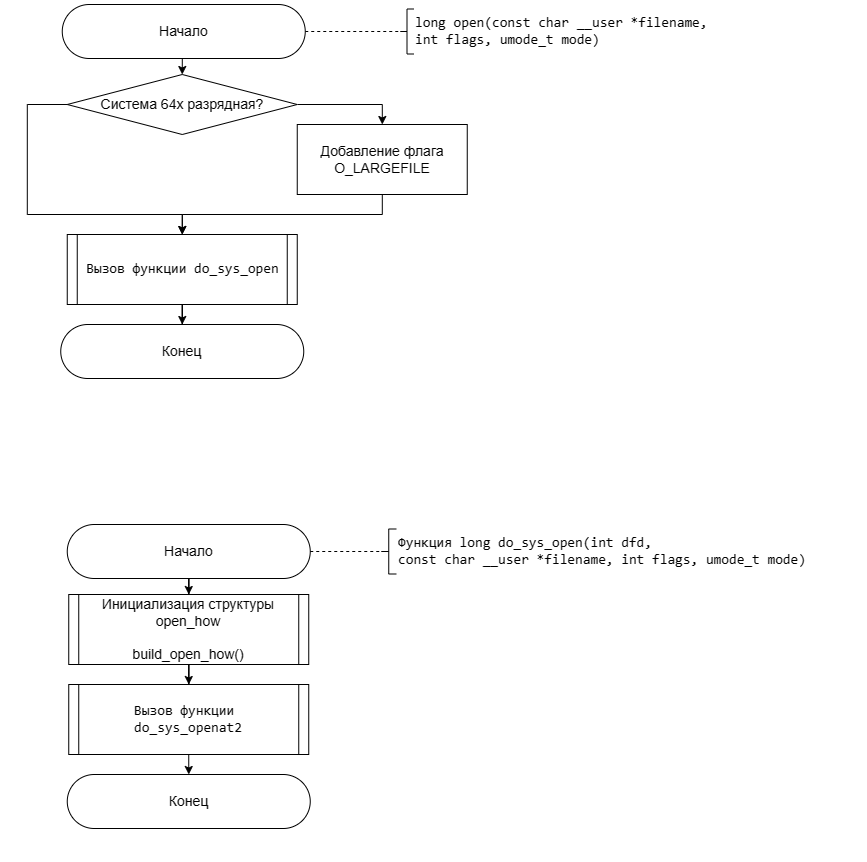
\includegraphics[scale=0.8]{do_sys_open1}
	\end{figure}

	\begin{figure}[H]
		\centering
		%\includegraphics[scale=0.45]{img/build_open_how.jpg}
	\end{figure}
	
	
	
	
	\section{build\_open\_how()}
	\begin{figure}[H]
		\centering
		\includegraphics[scale=0.55]{build_open_how}
	\end{figure}
	
	
	
	\section{do\_sys\_openat2()}
	\begin{figure}[H]
		\centering
		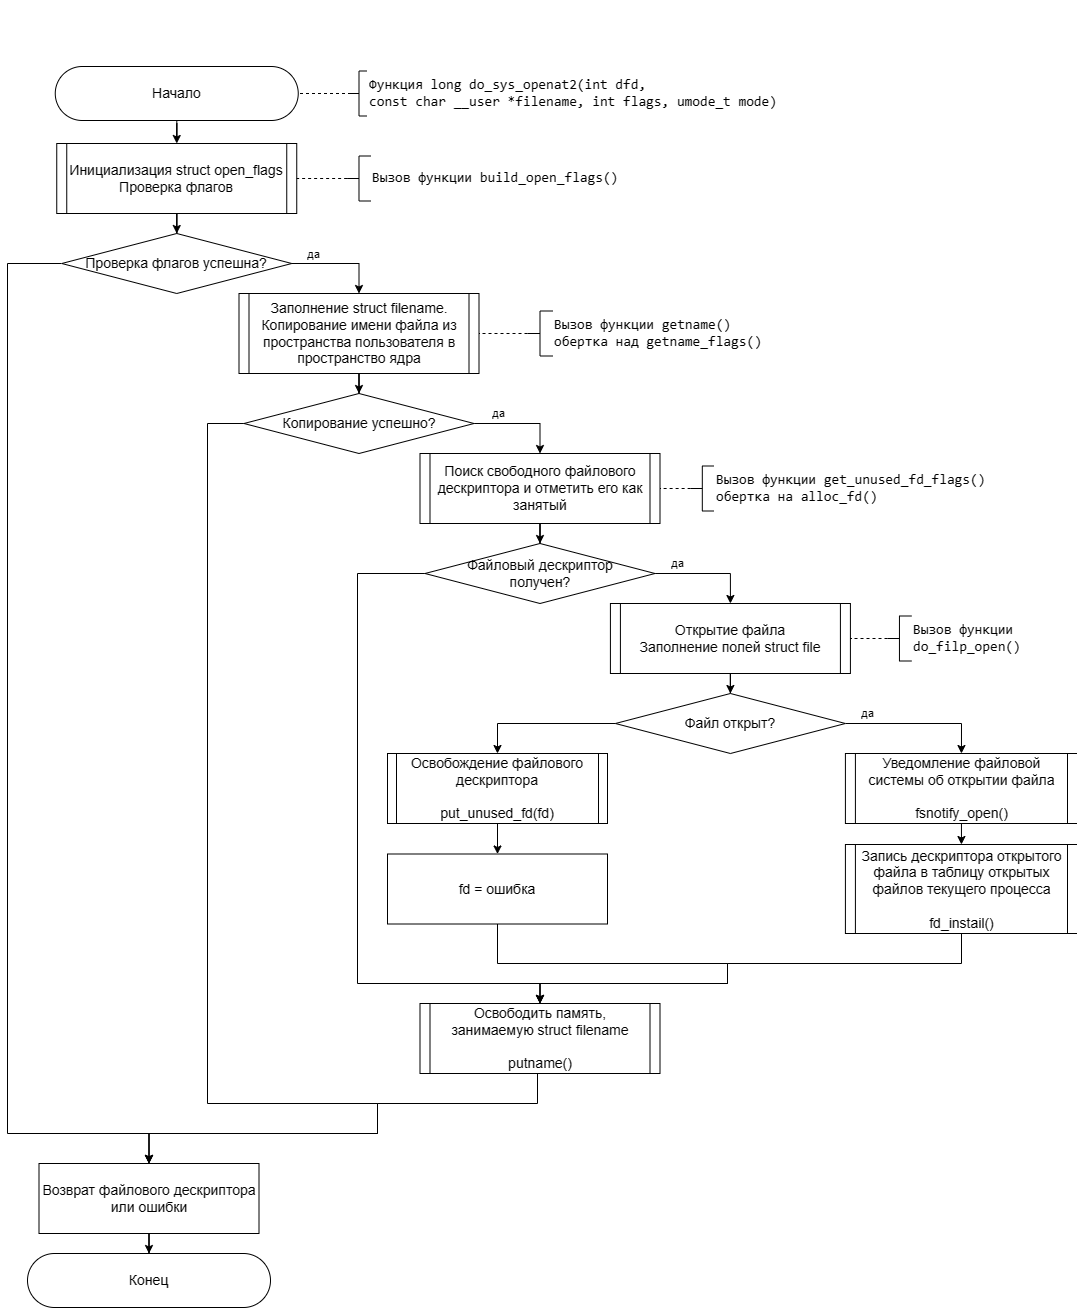
\includegraphics[scale=0.55]{do_sys_openat2}
	\end{figure}
	
	
	
	\section{build\_open\_flags()}
	
	
	\begin{figure}[H]
		\centering
		\includegraphics[scale=0.7]{build_open_flags1}
	\end{figure}

	\begin{figure}[H]
	\centering
	\includegraphics[scale=0.7]{build_open_flags2}
	\end{figure}
	
	\begin{figure}[H]
		\centering
		\includegraphics[scale=0.8]{build_open_flags3}
	\end{figure}
	
	\section{getname\_flags()}
	
	\begin{figure}[H]
		\centering
		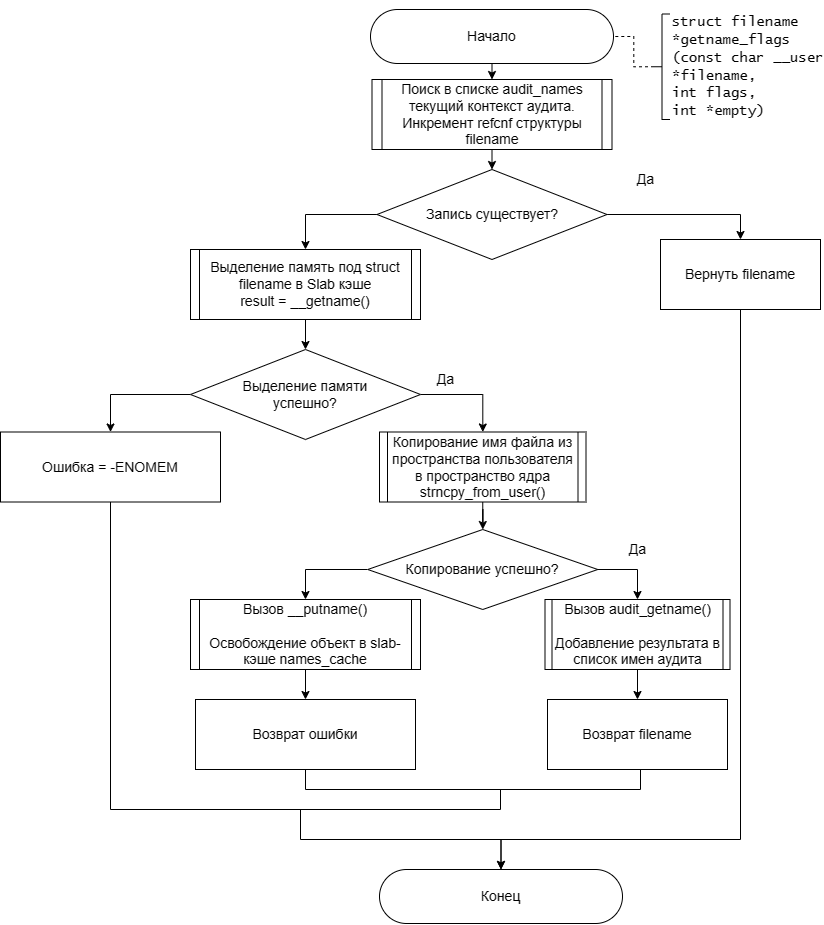
\includegraphics[scale=0.5]{get_name_flags}
	\end{figure}
	
	\section{alloc\_fd}
	
	\begin{figure}[H]
		\centering
		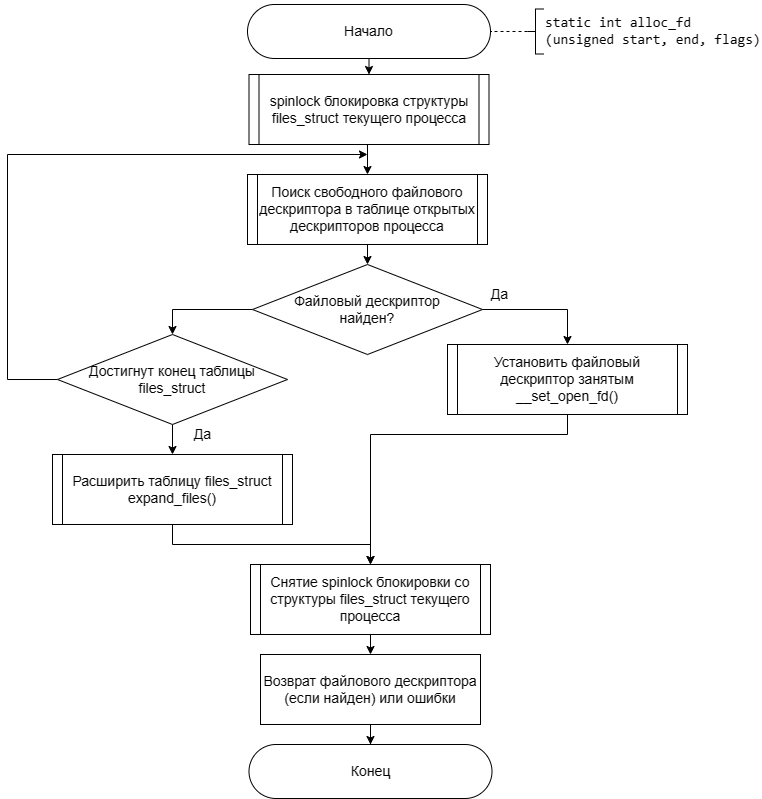
\includegraphics[scale=0.7]{alloc_fd}
	\end{figure}
	
	\section{do\_filp\_open}
	
	\begin{figure}[H]
		\centering		
		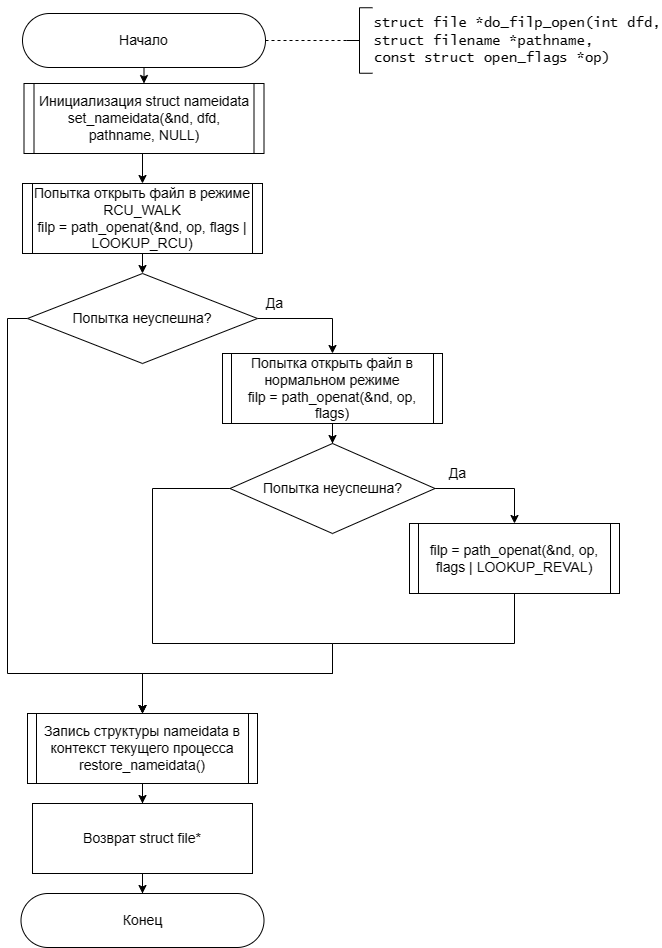
\includegraphics[scale=0.6]{do_filp_open}
	\end{figure}
	

	\section{path\_openat}
	
	\begin{figure}[H]
		\centering
		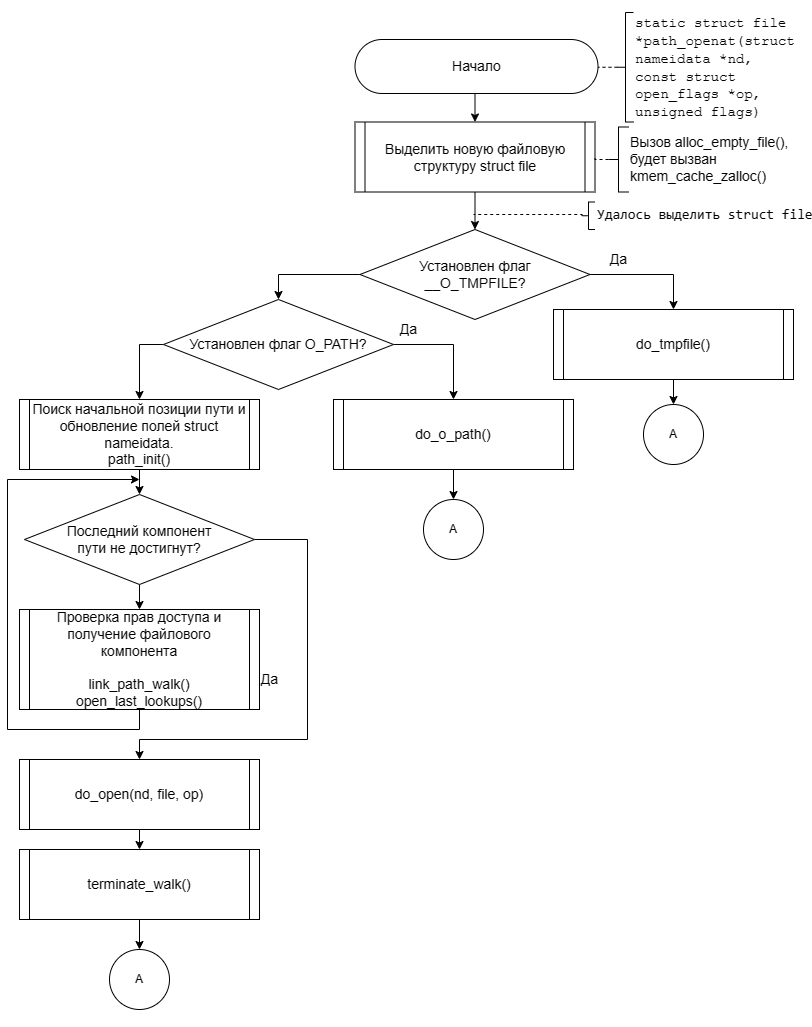
\includegraphics[scale=0.8]{path_openat1}
	\end{figure}
	
		\begin{figure}[H]
		\centering
		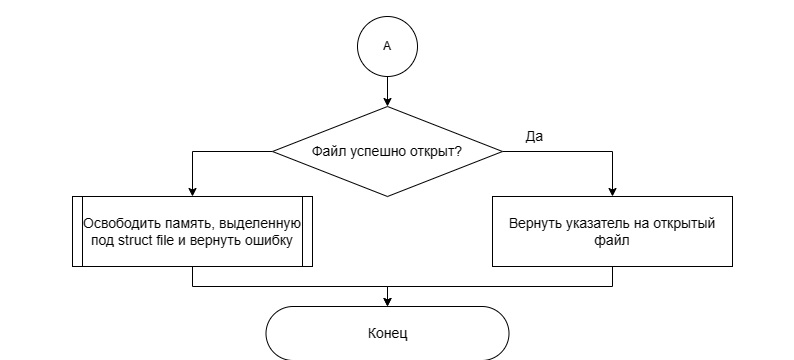
\includegraphics[scale=0.8]{path_openat2}
	\end{figure}
	
	\section{open\_last\_lookups}
	
	\begin{figure}[H]
		\centering
		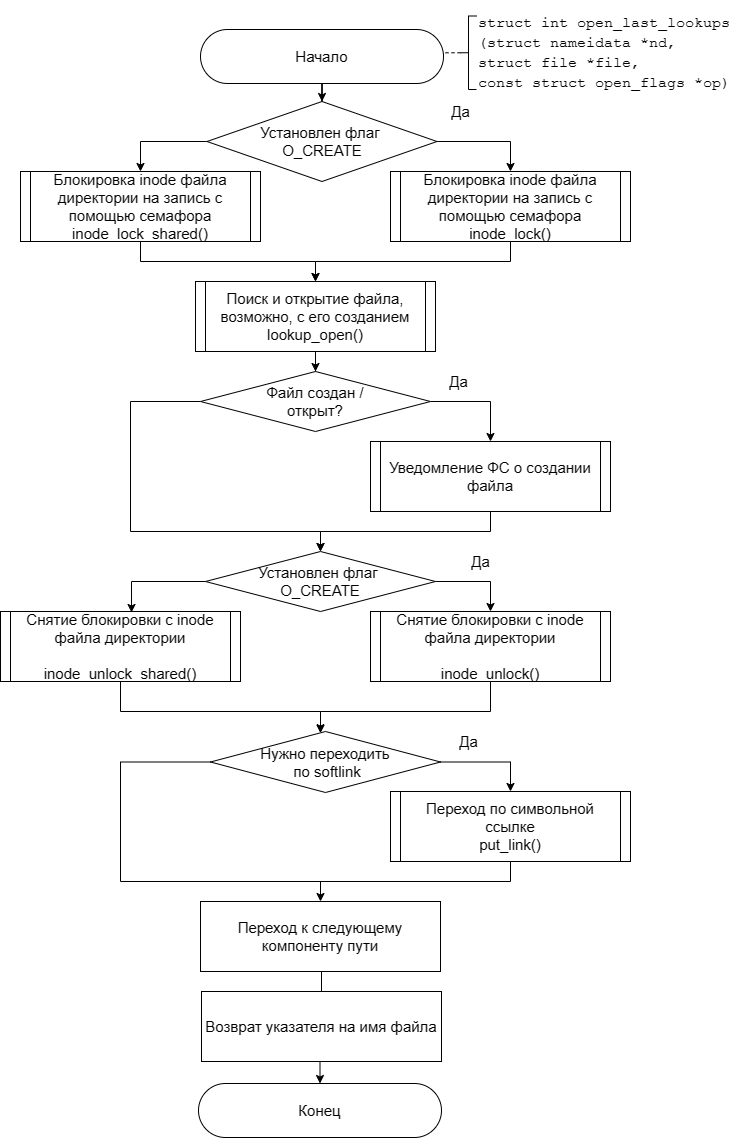
\includegraphics[scale=0.55]{open_last_lookups}
	\end{figure}
	
	\section{lookup\_open}
	
	\begin{figure}[H]
		\centering
		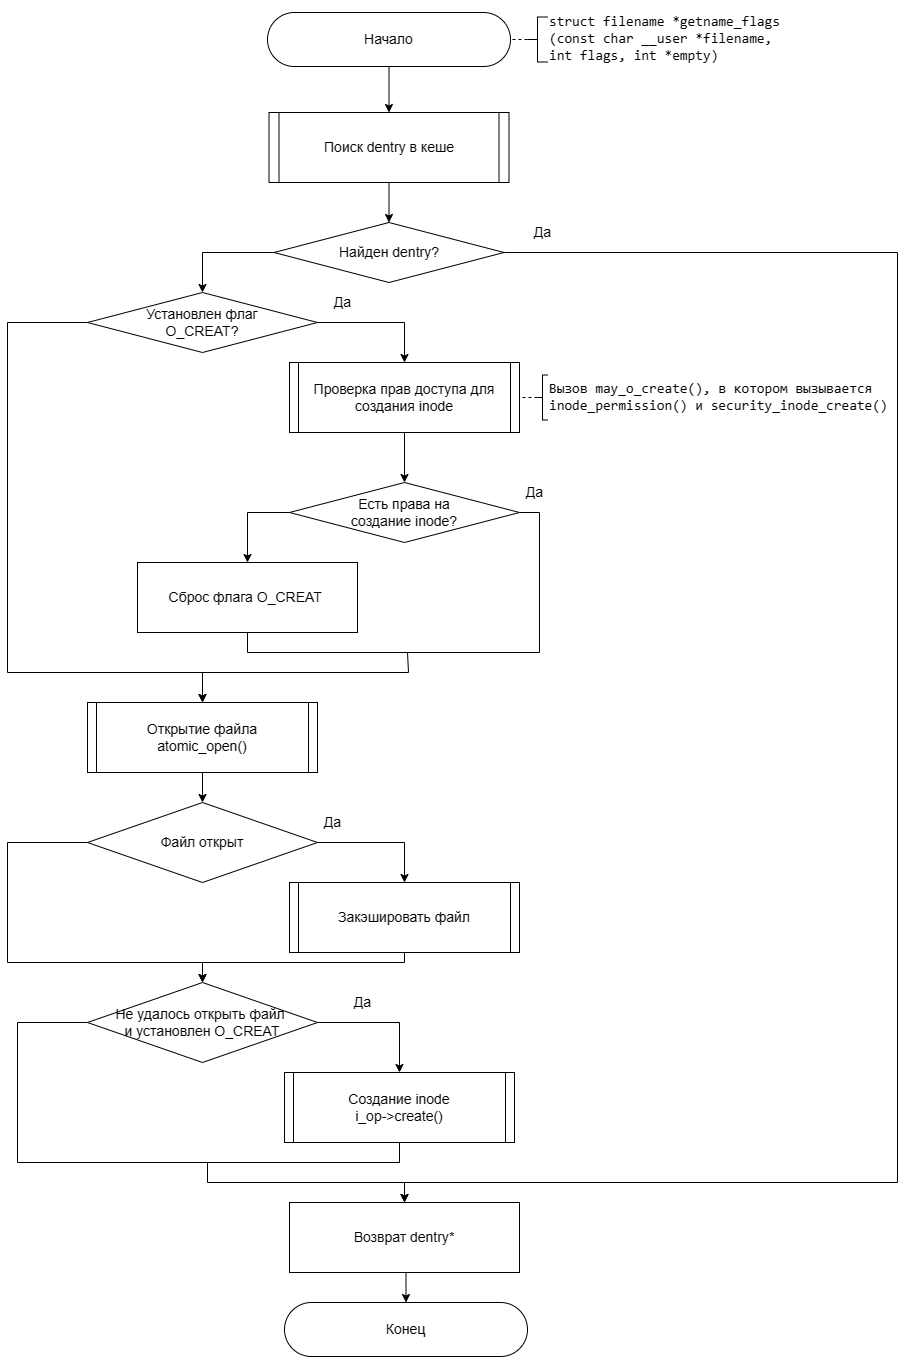
\includegraphics[scale=0.45]{lookup_open}
	\end{figure}
	
		\section{do\_open}
	
	\begin{figure}[H]
		\centering
		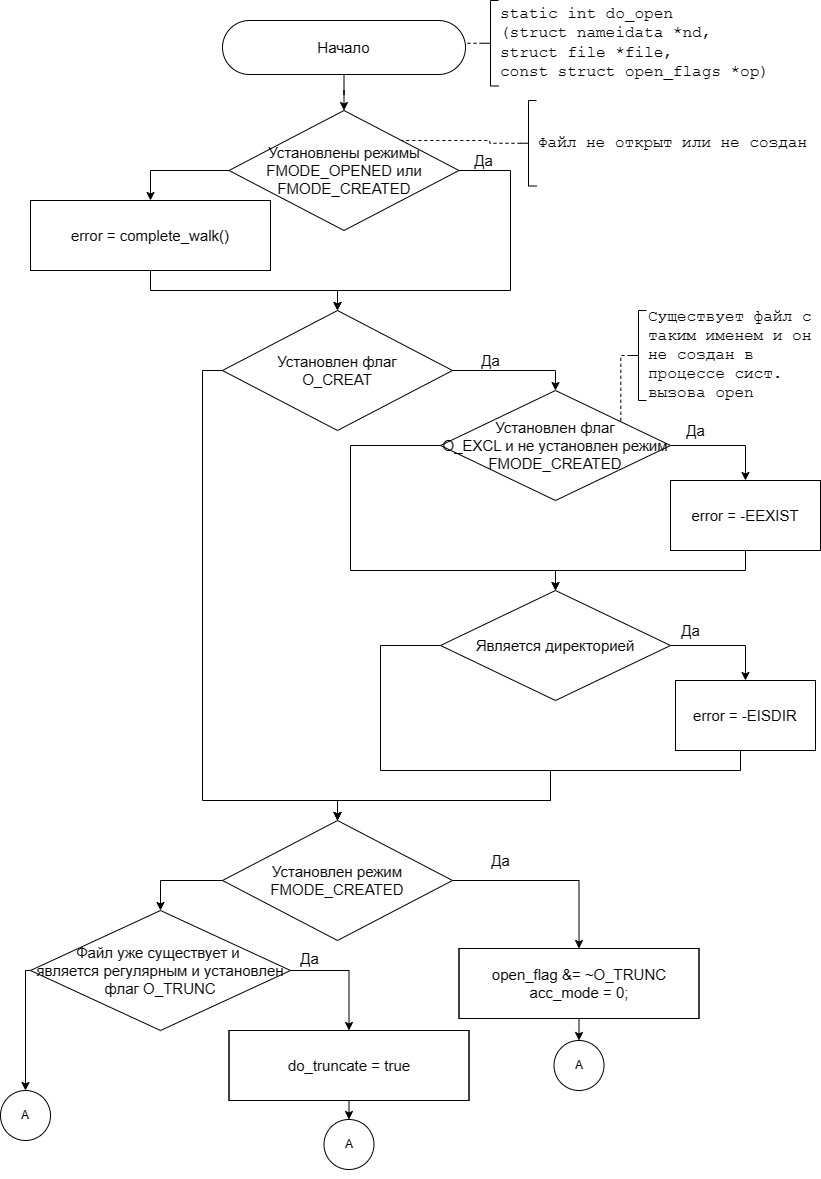
\includegraphics[scale=0.7]{do_open1}
	\end{figure}
	
		\begin{figure}[H]
		\centering
		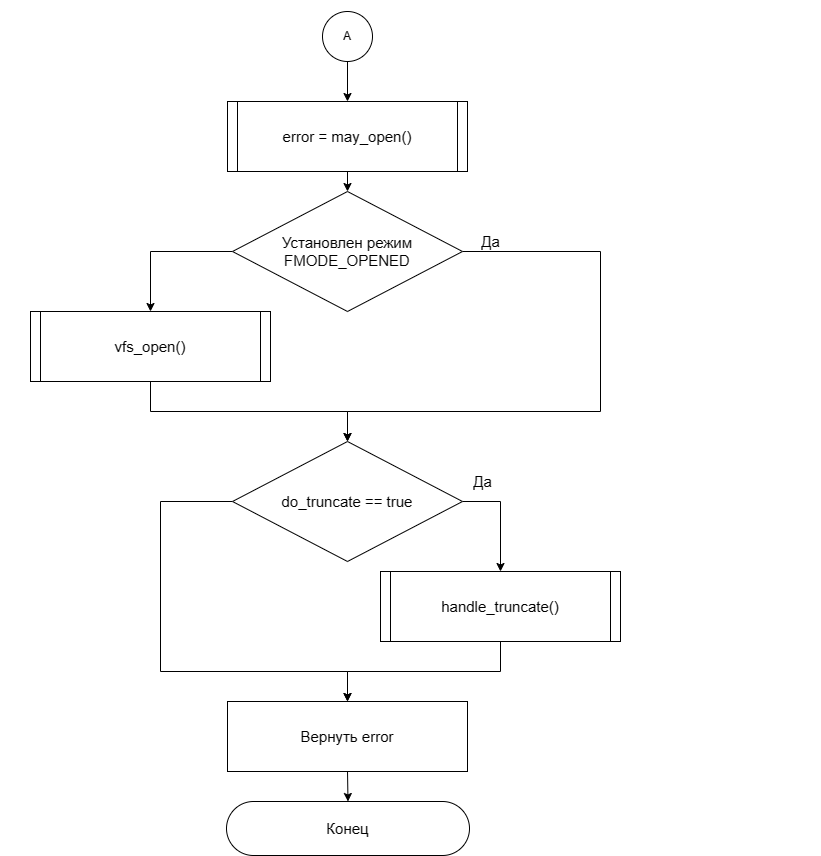
\includegraphics[scale=0.9]{do_open2}
	\end{figure}
	
	\section{set\_nameidata(), restore\_nameidata()}
	
			\begin{figure}[H]
		\centering
		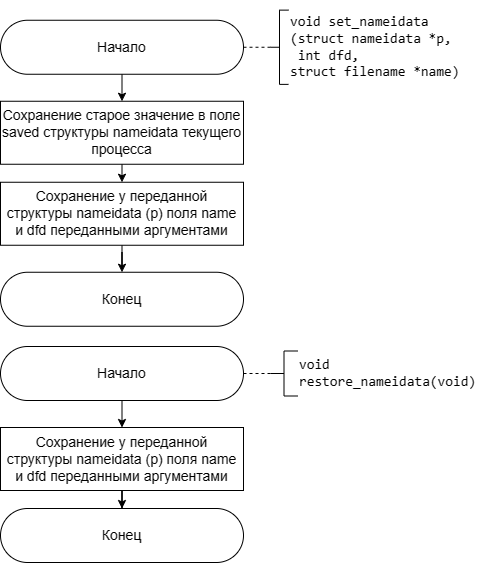
\includegraphics[scale=0.9]{set_nameidata}
	\end{figure}
	
	
	
	
	
	
	
	
	
	% \section{Схема работы алгоритма функции $\texttt{build\_open\_flags}$}
	
	%\begin{figure}[H]
	%	\centering
	%	\includegraphics[scale=0.5]{img/build_open_flags.jpg}
	%\end{figure}
	
	
	
	
	\bibliographystyle{utf8gost705u}  % стилевой файл для оформления по ГОСТу
	\bibliography{51-biblio}          % имя библиографической базы (bib-файла)
	
\end{document}
